\subsubsection{Rancangan Detail Komponen Konsensus}
\label{subsubsection:detail-komponen-konsensus}

Komponen konsensus bertanggung jawab untuk menjaga konsistensi data antar-\textit{Node} dalam sistem. Komponen ini akan mengimplementasikan algoritma konsensus yang diperlukan untuk mencapai kesepakatan di antara \textit{Node} dalam hal status dan nilai data seperti yang sudah dijelaskan di Bagian \ref{subsection:konsensus}.

Algoritma yang digunakan dalam komponen konsensus sesuai pertimbangan di Bagian \ref{subsubsection:pemilihan-algoritma-konsensus} adalah OmniPaxos. Algoritma ini diadaptasi untuk memenuhi kebutuhan spesifik dari sistem yang sedang dibangun, yaitu dengan menambahkan dukungan untuk \textit{erasure coding} dalam proses konsensus. OmniPaxos sudah memiliki desain yang modular sehingga memudahkan penyesuaian terhadap kebutuhan sistem. Ilustrasi struktur komponen konsensus dapat dilihat pada Gambar \ref{fig:consensus-component-structure}.

Kondisi yang disimpan oleh komponen konsensus terdapat pada bagian \textit{Sequence Paxos} yang berfungsi untuk menyimpan \textit{state} dari \textit{Node}, termasuk status \textit{leader}, \textit{follower}, \textit{log number}, dan informasi lainnya yang diperlukan untuk mencapai konsensus. Selain itu, OmniPaxos juga terhubung ke dalam sebuah penyimpanan data yang digunakan untuk menyimpan \textit{log} dari transaksi. Penyimpanan ini berbeda dengan \textit{Key-value store} yang digunakan oleh \textit{Node} untuk menyimpan data yang direplikasi atau di-\textit{erasure code}. Penyimpanan ini akan digunakan untuk menyimpan \textit{log} dari transaksi dan bersifat lokal, namun akan digunakan sebagai \textit{fallback} jika terjadi kegagalan pada \textit{Node}.

Selain itu, komponen OmniPaxos bertanggung jawab untuk melakukan operasi \textit{erasure coding} pada data jika sistem menggunakan skema tersebut. Skema \textit{erasure coding} menyebabkan data yang ditransaksikan menjadi tidak sama antara \textit{Node} yang satu dengan yang lainnya. Penggunaan \textit{erasure coding} juga mengubah jumlah \textit{Node} yang diperlukan untuk mencapai kuorum, mengikuti referensi pada Bagian \ref{subsection:paxos-erasure}. Dengan demikian, lebih mudah jika komponen \textit{erasure coding} berada pada komponen utama yang berkaitan dengan konsensus. Komponen \textit{erasure coding service} akan menyimpan konfigurasi \textit{data shard} dan \textit{parity shard} yang digunakan untuk melakukan operasi \textit{erasure coding}. Komponen ini juga melakukan operasi \textit{erasure coding} pada data yang diterima dari \textit{Node} dan mengembalikan hasilnya ke \textit{Node}.

\begin{figure}[ht]
    \centering
    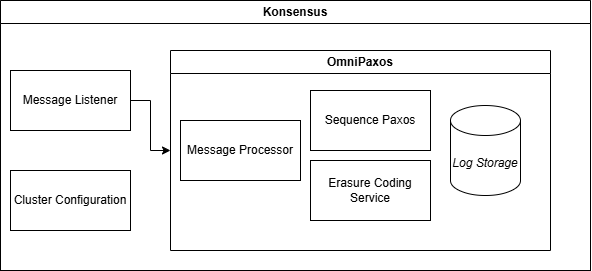
\includegraphics[width=0.85\textwidth]{resources/chapter-3/consensus-architecture.png}
    \caption{Struktur Komponen Konsensus}
    \label{fig:consensus-component-structure}
\end{figure}
